\documentclass[a4paper]{article}
\usepackage{amsfonts}
\usepackage{amsmath}
\usepackage{amssymb}
\usepackage{graphicx} 
\usepackage{cancel}

\begin{document}
  
\noindent \large Auteur: Odia Kibor \\
\noindent \large Studierichting: Informatica\\
\noindent \large Oefeningenreeks 5G nr. 6.2
\\

\medskip

\normalsize


$ f(x) = \sqrt{x} $\\

$ g(x) = 2\sqrt[4]{x} $\\

$ f(x) = g(x) $\\

$ \sqrt{x} = 2\sqrt[4]{x} $\\

$ \Leftrightarrow x^{\frac{1}{2}} = 2x^{\frac{1}{4}} $\\

$ \Leftrightarrow x^{\frac{1}{2}} - 2x^{\frac{1}{4}} = 0 $\\

$ \Leftrightarrow x^{\frac{1}{4}}\left(x^{\frac{1}{4}} - 2\right) = 0 $\\

$ \Leftrightarrow x^{\frac{1}{4}} = 0 \text{ of } x^{\frac{1}{4}} = 2 $\\

$ \Leftrightarrow x = 0 \text{ of } x = 16 $\\

$\Rightarrow x \in [0, 16]$\\

We testen een punt tussen $0$ en $16$: $x = 1$\\

$ f(1) = \sqrt{1} = 1 $\\

$ g(1) = 2\sqrt[4]{1} = 2 $\\

$\Rightarrow g(x)$ is de bovenste functie\\

$\Rightarrow V = \pi \displaystyle\int_0^{16} \left(g(x)^2 - f(x)^2\right)dx$\\

$= \pi \displaystyle\int_0^{16} \left((2\sqrt[4]{x})^2 - (\sqrt{x})^2\right)dx$\\

$(2\sqrt[4]{x})^2 = 4x^{\frac{1}{2}}$\\

$(\sqrt{x})^2 = x$\\

$\Rightarrow (2\sqrt[4]{x})^2 - (\sqrt{x})^2 = 4x^{\frac{1}{2}} - x$\\

$\Rightarrow V = \pi \displaystyle\int_0^{16} \left(4x^{\frac{1}{2}} - x\right)dx$\\

$= \pi \left[\dfrac{4x^{\frac{3}{2}}}{\frac{3}{2}} - \dfrac{x^2}{2}\right]_0^{16}$\\

$= \pi \left[\dfrac{8}{3}x^{\frac{3}{2}} - \dfrac{x^2}{2}\right]_0^{16}$\\

$= \pi \left(\dfrac{8}{3}(16)^{\frac{3}{2}} - \dfrac{16^2}{2}\right) - \pi \left(\dfrac{8}{3}(0)^{\frac{3}{2}} - \dfrac{0^2}{2}\right)$\\

$16^{\frac{3}{2}} = \left(\sqrt{16}\right)^3 = 4^3 = 64$\\

$\Rightarrow V = \pi \left(\dfrac{8}{3}\cdot 64 - \dfrac{256}{2}\right) - \pi(0)$\\

$= \pi \left(\dfrac{512}{3} - 128\right)$\\

$= \pi \left(\dfrac{512}{3} - \dfrac{384}{3}\right)$\\

$= \pi \cdot \dfrac{128}{3}$\\

$\Rightarrow V = \dfrac{128\pi}{3}$\\

\begin{figure}[h]
\centering
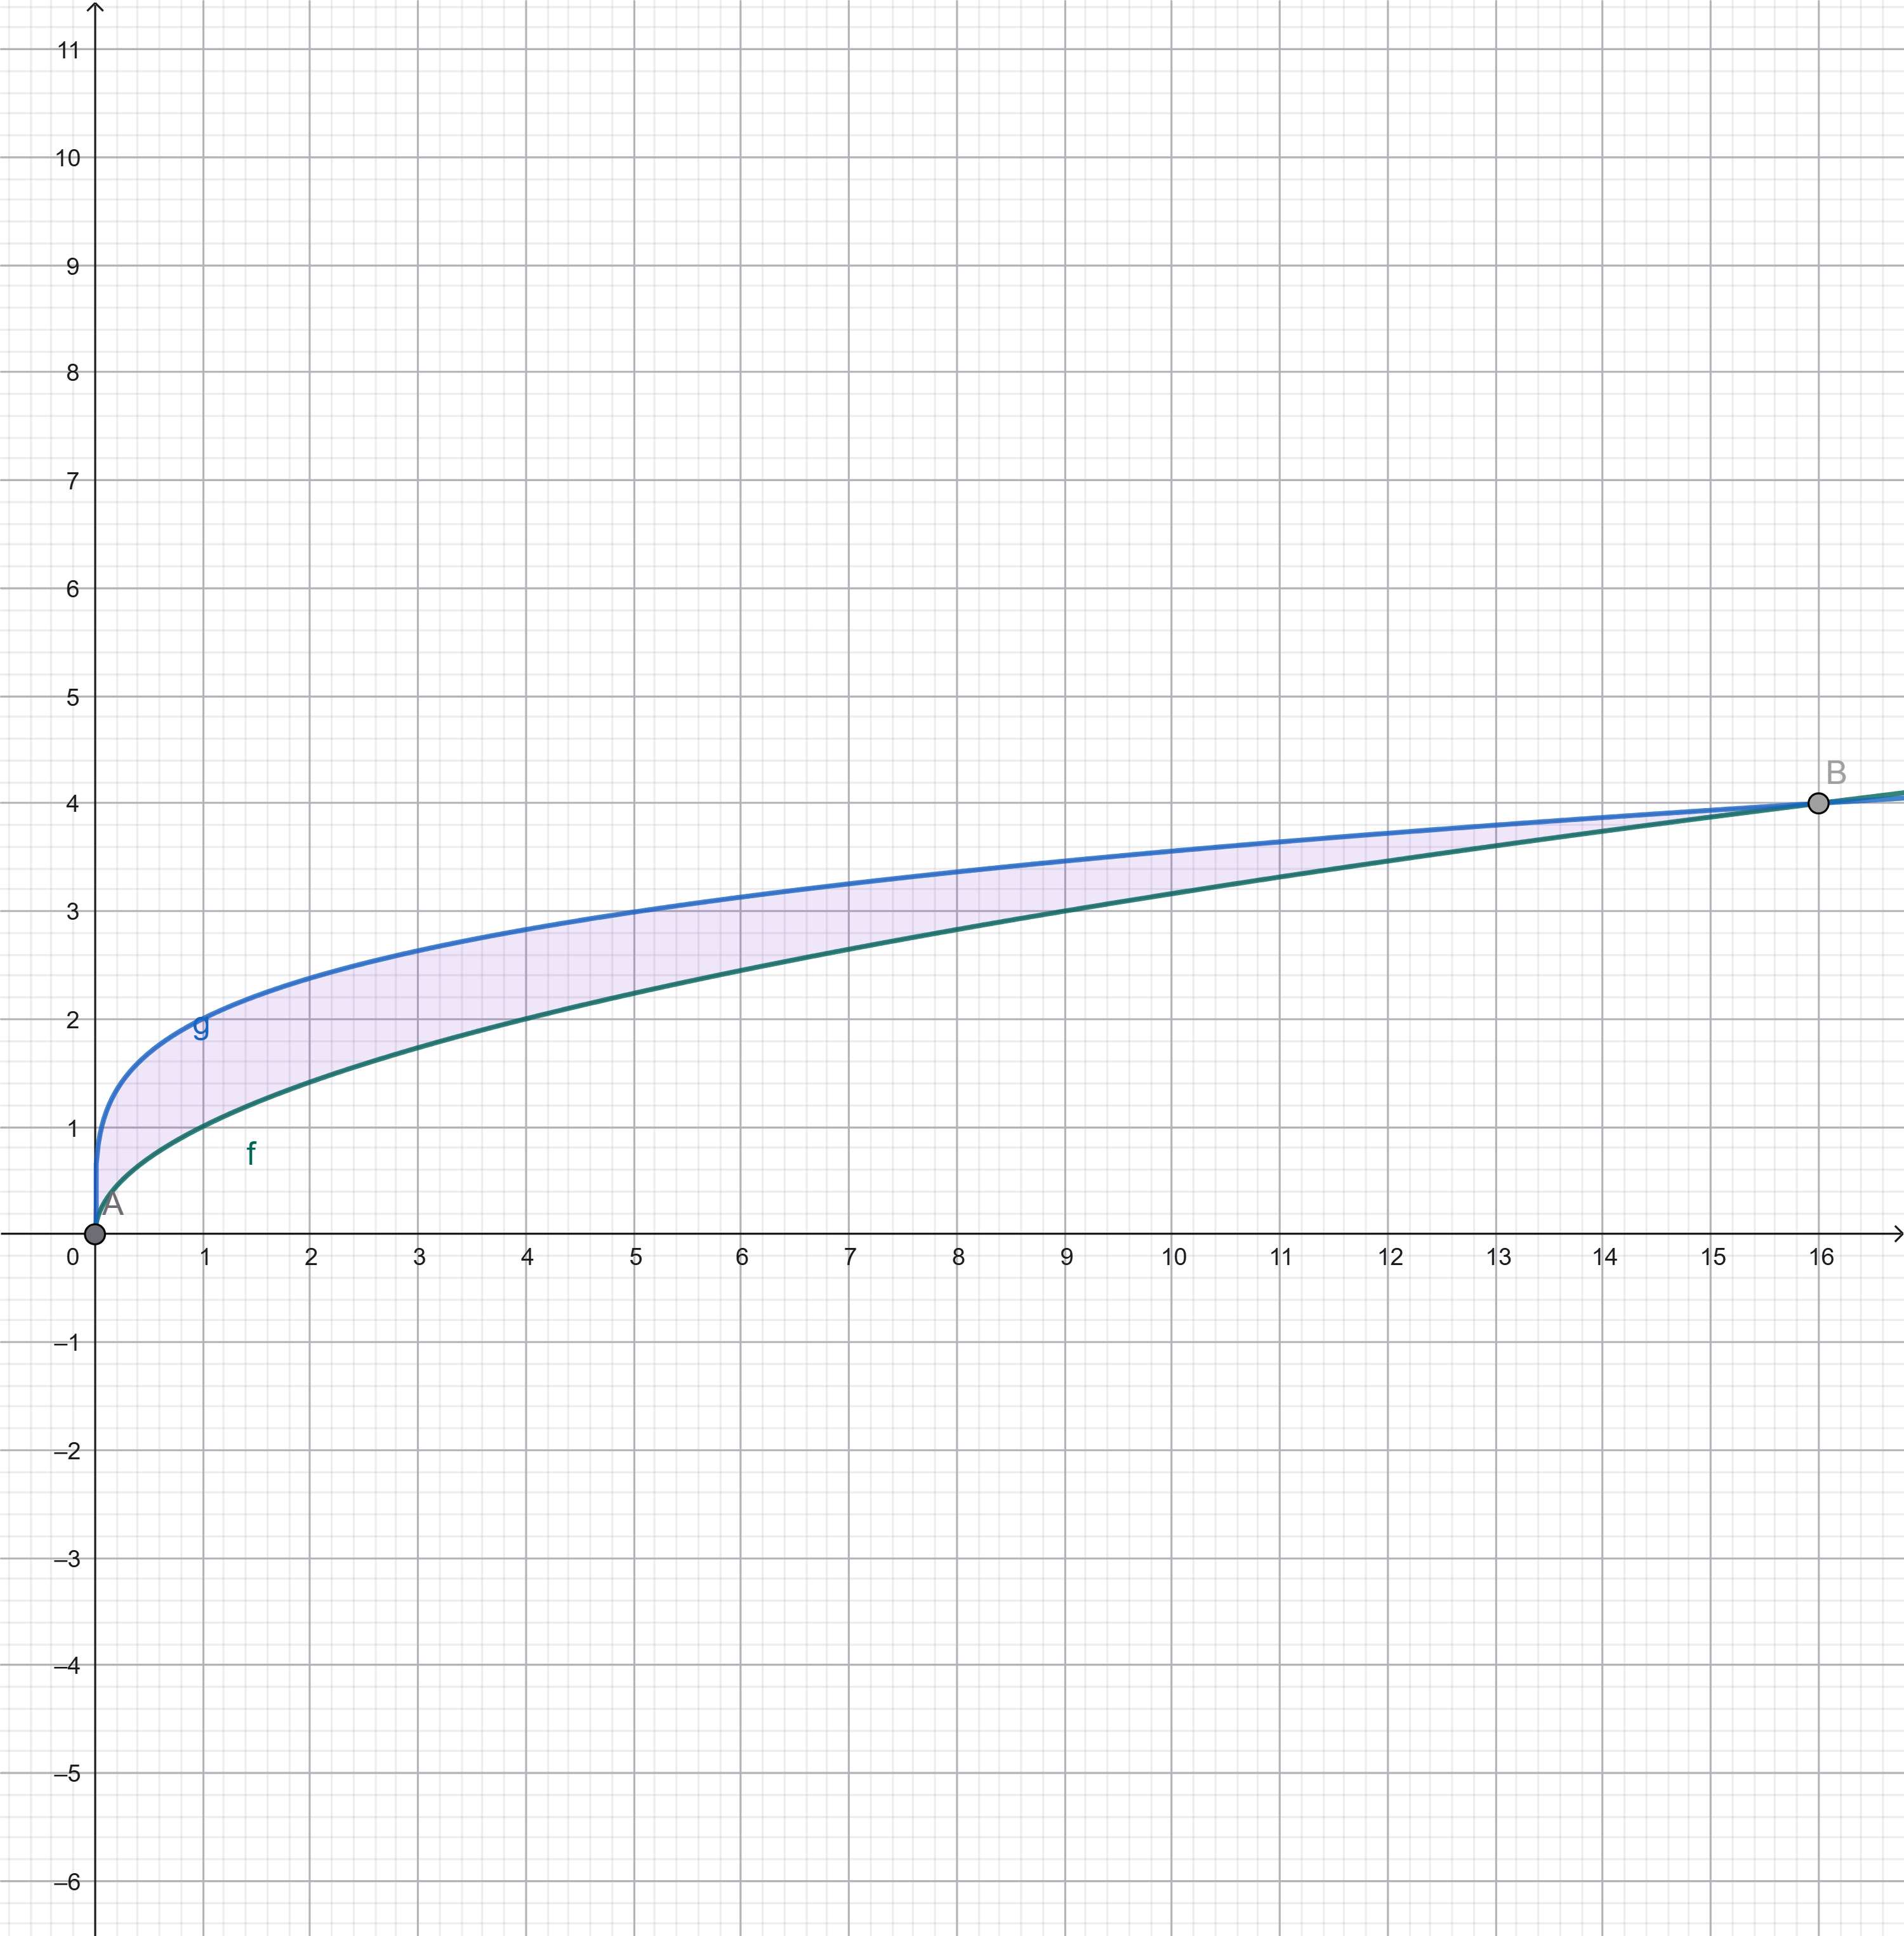
\includegraphics[width=5cm]{5G-6.2-odia.kibor.INF.png}
\end{figure}




















\begin{thebibliography}{999}
%\bibitem{a} Referentie
\end{thebibliography}
\end{document} 


